\chapter{EEXCESS-Browser}

\section{Erstellung des Sechobjects}

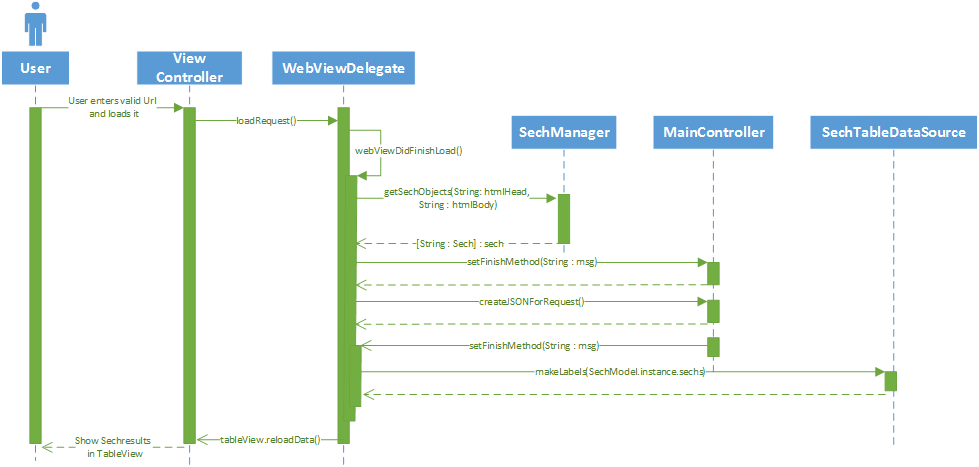
\includegraphics[scale=1]{sechobject.png}

Ablauf:
Sobald der User eine gültige URL eingibt und lädt, wird die Laderoutine (loadRequest())
angestoßen. Ist die Seite fertig geladen wird in der Delegatemethode webViewDidFinishLoad()
des WebViewDelegates das Auslesen bzw. Laden der Sechtags begonnen.
Dem SechManager wird der HTML-Head und –Body der eben geladenen Website übergeben und es
werden mit Hilfe des HTMLManagers Sechobjekte erstellt. Diese Sechobjekte werden in einem
Dictionary zurückgegeben.
Die setFinishMethod()-Methode bereitet den MainController darauf vor, asynchron eine Methode
im WebViewDelegate aufzurufen, sobald die Sechobjekte durch die Response erweitert worden
sind. Der Prozess der EEXCESS-Abfrage wird dann durch die Methode createJSONForRequest() mit
dem Parameter des Sechdictionarys angestoßen. Sobald dann die Elemente erweitert wurden ruft
der MainController die setFinishMethod() des WebViewDelegates auf und die Liste der Sechtags
im UI wird aktualisiert.
